\section{Second strategy}

As in the previous strategy, Alice will once again need an order satisfying $col_{2}(G)$.
Using this order, she will achieve her own coloring of the graph (without any intervention from Bob).
This coloration must comply with the following rules:
\begin{itemize}
\item A vertex must not have the same color as its loose backward neighbors.
\item Vertices forming a cycle must be colored with at least 3 colors.
\item This coloring must use at most $col_{2}(G)$ colors.
\end{itemize}

We will call the resulting graph $G'$.

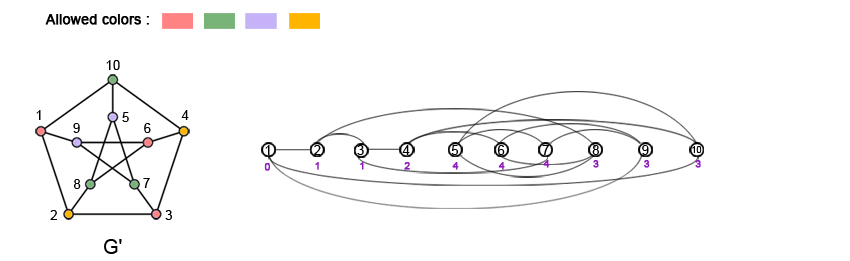
\includegraphics[width=13cm]{gameS2t1.jpg}

Now Alice will use $G'$ to provide guidance in the coloring of the graph $G$. For each bicolor subgraph of $G'$,
we direct the edges such that each vertex has an out-degree of no more than $1$. 

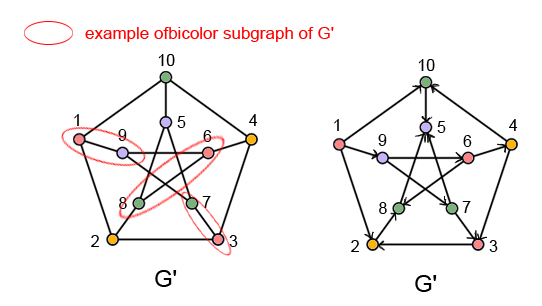
\includegraphics[width=8cm]{gameS2t2.jpg}

As each edge appears only in
one subgraph, we know that we oriented the entire graph $G$. We can now begin the game. 
A vertex $v$ (colored with a color $c$ on the graph $G'$) is endangered if one of its incoming neighbors is colored in a shade of $c$. Alice coloring the graph in accordance with the coloring of $G'$, a vertex can only be endangered by Bob. In addition, the orientation of $G'$ is such that there can be only one vertex in danger per round.

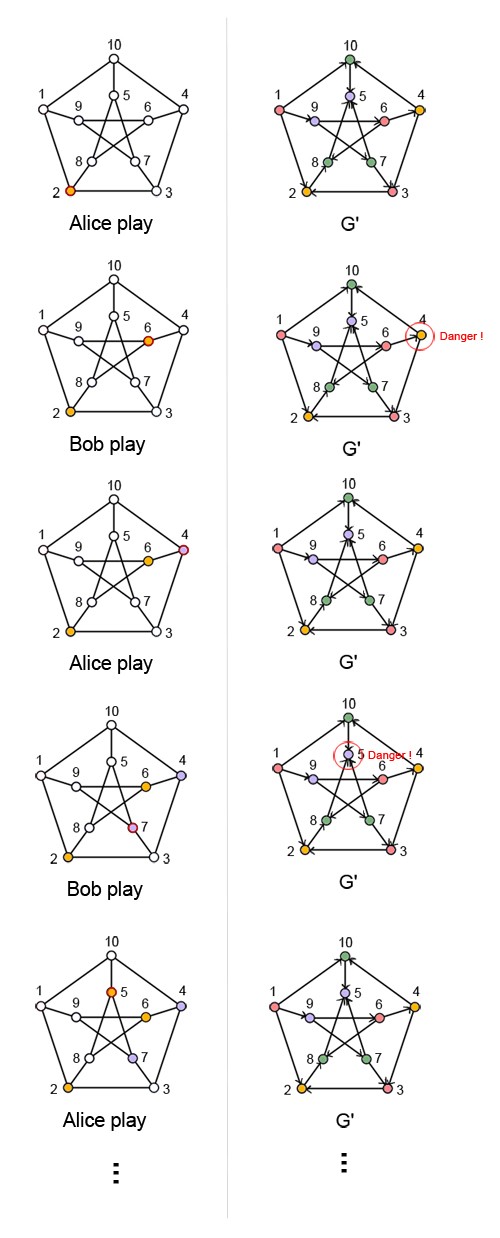
\includegraphics[width=8cm]{gameS2t3.jpg}

According to this strategy, each graph satisfies $\chi_{g}(G) \leq a(G) \times (a(G) + 1)$, where $a(G)$, the acyclic chromatic number of $G$, is the minimum number of colors used on $G$ such that each cycle is colored with at least $3$ colors.